% Figure 5: The Evans-Jost mechanism: outgoing/decaying columns, the
% determinant condition, and the rank-one resolvent residue.
% Authors: Dr. Davide Batic and Dr. Denys Dutykh
%          (Mathematics Department, Khalifa University of Science and
%           Technology, Abu Dhabi, UAE)
\documentclass[tikz,border=6pt]{standalone}
% ============================================================================
% Shared TikZ style for the figures of the Kerr–Dirac two-channel scattering
% manuscript (compiled standalone into ../latex/figures/).
% Authors: Dr. Davide Batic and Dr. Denys Dutykh
%          (Mathematics Department, Khalifa University of Science and
%           Technology, Abu Dhabi, UAE)
%
% Visual language (used consistently across all figures):
%   * horizon channel      : navy  (chH)
%   * spatial-infinity     : teal  (chI)
%   * accents / emphasis   : gold  (acc)
%   * future/out data      : solid arrows
%   * past/in data         : dashed arrows
%   * proved here          : solid box border
%   * imported input       : light-gray filled box
%   * conditional          : dashed box border
% ============================================================================
\usepackage{amsmath,amssymb}
\usetikzlibrary{arrows.meta,positioning,decorations.pathmorphing,calc,matrix}

\definecolor{chH}{HTML}{142D6E}   % horizon channel (navy)
\definecolor{chI}{HTML}{0E6E6E}   % spatial-infinity channel (teal)
\definecolor{acc}{HTML}{9A7A2E}   % gold accent
\definecolor{warm}{HTML}{9C5310}  % sienna (warnings/exclusions)
\definecolor{ltg}{HTML}{F2F2F2}   % light gray fill (imported)

\tikzset{
  outarr/.style={-{Stealth[length=2.6mm]}, line width=0.9pt},
  inarr/.style={-{Stealth[length=2.6mm]}, line width=0.9pt, dashed},
  axis/.style={-{Stealth[length=2.2mm]}, line width=0.6pt, gray!70!black},
  wavyH/.style={chH, decorate, decoration={snake, amplitude=0.45mm, segment length=2.6mm}},
  wavyI/.style={chI, decorate, decoration={snake, amplitude=0.45mm, segment length=2.6mm}},
  proved/.style={draw, line width=0.7pt, rounded corners=2pt, inner sep=4pt},
  imported/.style={draw=gray!60, fill=ltg, line width=0.5pt, rounded corners=2pt, inner sep=4pt},
  conditional/.style={draw, dashed, line width=0.7pt, rounded corners=2pt, inner sep=4pt},
  lab/.style={font=\small},
  slab/.style={font=\footnotesize},
  tlab/.style={font=\scriptsize},
}

\begin{document}
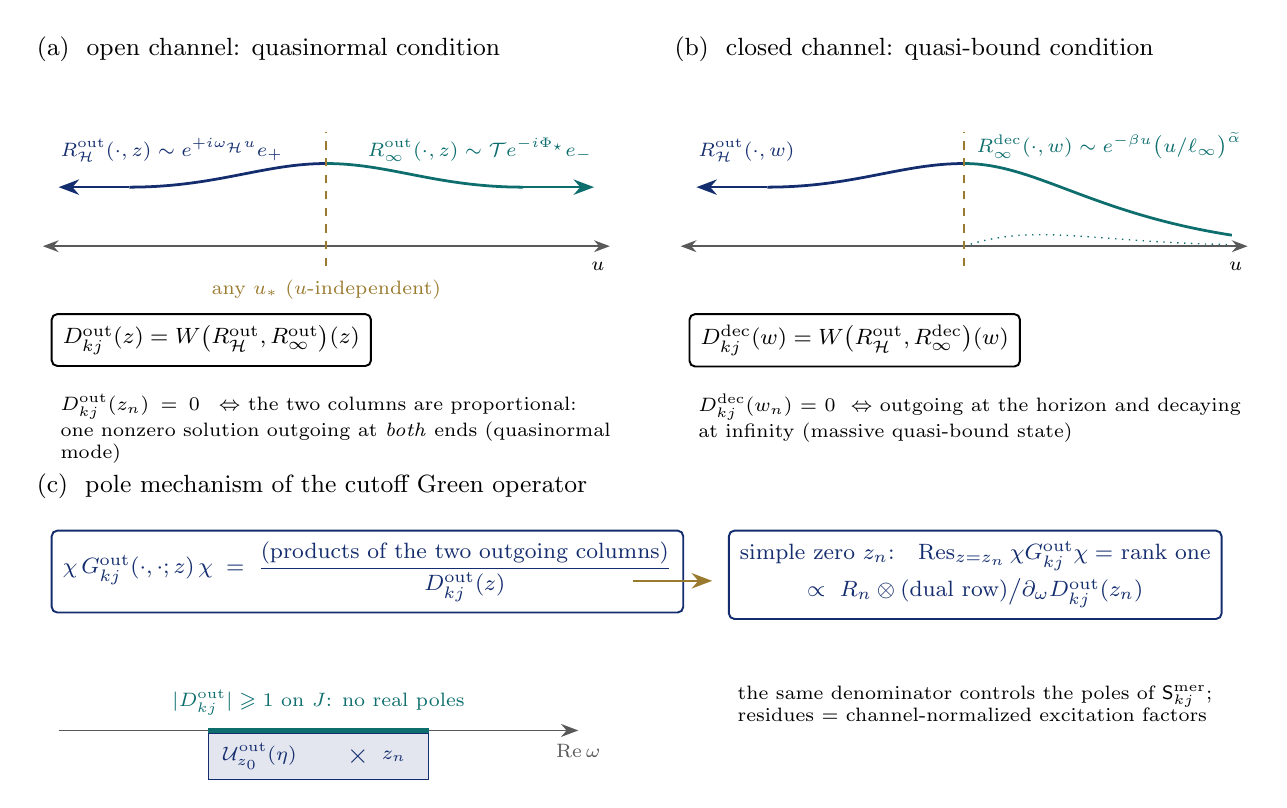
\begin{tikzpicture}[x=1cm,y=1cm]

% ============ panel (a): open channel, quasinormal condition ===============
\begin{scope}[shift={(0,0)}]
  \node[lab, anchor=west] at (-0.4,2.5) {(a)\ \ open channel: quasinormal condition};
  \draw[axis, {Stealth[length=2mm]}-{Stealth[length=2mm]}] (-0.2,0) -- (7.0,0);
  \node[tlab, anchor=north] at (6.85,-0.08) {$u$};
  % horizon outgoing column: control toward the horizon, integrated to u*
  \draw[outarr, chH] (0.9,0.75) -- (0.0,0.75);
  \draw[chH, line width=1.0pt]
    (0.9,0.75) .. controls (2.0,0.75) and (2.6,1.05) .. (3.4,1.05);
  \node[tlab, chH, anchor=south west] at (-0.1,0.95)
    {$R_{\mathcal H}^{\rm out}(\cdot,z)\sim e^{+i\omega_{\mathcal H}u}e_+$};
  % infinity outgoing column
  \draw[outarr, chI] (5.9,0.75) -- (6.8,0.75);
  \draw[chI, line width=1.0pt]
    (5.9,0.75) .. controls (4.8,0.75) and (4.2,1.05) .. (3.4,1.05);
  \node[tlab, chI, anchor=south east] at (6.9,0.95)
    {$R_\infty^{\rm out}(\cdot,z)\sim\mathcal Te^{-i\Phi_\star}e_-$};
  % matching point
  \draw[acc, dashed, line width=0.7pt] (3.4,-0.25) -- (3.4,1.45);
  \node[tlab, acc, anchor=north] at (3.4,-0.30) {any $u_*$ ($u$-independent)};
  \node[proved, slab, anchor=north west] at (-0.1,-0.85)
    {$D^{\rm out}_{kj}(z)=W\bigl(R_{\mathcal H}^{\rm out},R_\infty^{\rm out}\bigr)(z)$};
  \node[tlab, anchor=north west, text width=7.0cm] at (-0.1,-1.75)
    {$D^{\rm out}_{kj}(z_n)=0\ \Leftrightarrow$ the two columns are proportional:
     one nonzero solution outgoing at \emph{both} ends (quasinormal mode)};
\end{scope}

% ============ panel (b): closed channel, quasi-bound condition ==============
\begin{scope}[shift={(8.1,0)}]
  \node[lab, anchor=west] at (-0.4,2.5) {(b)\ \ closed channel: quasi-bound condition};
  \draw[axis, {Stealth[length=2mm]}-{Stealth[length=2mm]}] (-0.2,0) -- (7.0,0);
  \node[tlab, anchor=north] at (6.85,-0.08) {$u$};
  \draw[outarr, chH] (0.9,0.75) -- (0.0,0.75);
  \draw[chH, line width=1.0pt]
    (0.9,0.75) .. controls (2.0,0.75) and (2.6,1.05) .. (3.4,1.05);
  \node[tlab, chH, anchor=south west] at (-0.1,0.95)
    {$R_{\mathcal H}^{\rm out}(\cdot,w)$};
  % decaying infinity column with shrinking envelope
  \draw[chI, line width=1.0pt]
    (3.4,1.05) .. controls (4.3,1.05) and (5.0,0.42) .. (6.8,0.14);
  \draw[chI, line width=0.5pt, dotted]
    (3.4,-0.0) .. controls (4.3,0.30) and (5.0,0.05) .. (6.8,0.02);
  \node[tlab, chI, anchor=south east, align=right] at (7.05,0.98)
    {$R_\infty^{\rm dec}(\cdot,w)\sim e^{-\beta u}\bigl(u/\ell_\infty\bigr)^{\widetilde\alpha}$};
  \draw[acc, dashed, line width=0.7pt] (3.4,-0.25) -- (3.4,1.45);
  \node[proved, slab, anchor=north west] at (-0.1,-0.85)
    {$D^{\rm dec}_{kj}(w)=W\bigl(R_{\mathcal H}^{\rm out},R_\infty^{\rm dec}\bigr)(w)$};
  \node[tlab, anchor=north west, text width=7.0cm] at (-0.1,-1.75)
    {$D^{\rm dec}_{kj}(w_n)=0\ \Leftrightarrow$ outgoing at the horizon and decaying
     at infinity (massive quasi-bound state)};
\end{scope}

% ============ panel (c): the resolvent pole mechanism =======================
\begin{scope}[shift={(0,-4.6)}]
  \node[lab, anchor=west] at (-0.4,1.55) {(c)\ \ pole mechanism of the cutoff Green operator};
  \node[proved, chH, slab, align=center, anchor=north west] at (-0.1,1.0)
    {$\chi\,G^{\rm out}_{kj}(\cdot,\cdot;z)\,\chi\;=\;
      \dfrac{\hbox{(products of the two outgoing columns)}}{D^{\rm out}_{kj}(z)}$};
  \draw[outarr, acc] (7.3,0.35) -- (8.3,0.35);
  \node[proved, chH, slab, align=center, anchor=north west] at (8.5,1.0)
    {simple zero $z_n$:\quad
     $\operatorname*{Res}_{z=z_n}\chi G^{\rm out}_{kj}\chi=$ rank one\\[0.6mm]
     $\propto\ R_n\otimes(\hbox{dual row})\big/\partial_\omega D^{\rm out}_{kj}(z_n)$};
  % mini omega-plane
  \begin{scope}[shift={(3.2,-1.55)}]
    \draw[axis] (-3.2,0) -- (3.4,0) node[tlab, anchor=north, yshift=-0.5mm] {$\operatorname{Re}\omega$};
    \draw[chI, line width=1.8pt] (-1.3,0) -- (1.5,0);
    \node[tlab, chI, anchor=south] at (0.1,0.07) {$|D^{\rm out}_{kj}|\geqslant1$ on $J$: no real poles};
    \fill[chH!12] (-1.3,-0.62) rectangle (1.5,-0.04);
    \draw[chH, line width=0.5pt] (-1.3,-0.62) rectangle (1.5,-0.04);
    \node[chH] at (0.6,-0.33) {$\times$};
    \node[tlab, chH, anchor=west] at (0.78,-0.33) {$z_n$};
    \node[tlab, chH, anchor=east] at (-0.05,-0.33) {$\mathcal U^{\rm out}_{z_0}(\eta)$};
  \end{scope}
  \node[tlab, anchor=north west, text width=6.2cm] at (8.5,-0.85)
    {the same denominator controls the poles of $\mathsf S^{\rm mer}_{kj}$;
     residues $=$ channel-normalized excitation factors};
\end{scope}

\end{tikzpicture}
\end{document}
